\documentclass{article}
\usepackage{amsmath}
\usepackage{graphicx}
\usepackage{graphics}
\usepackage{amssymb}
\usepackage{booktabs}
\usepackage{listings}
\usepackage{color}
\usepackage{caption}
\usepackage{subcaption}
\usepackage[margin=0.8in]{geometry}

\definecolor{dkgreen}{rgb}{0,0.6,0}
\definecolor{gray}{rgb}{0.5,0.5,0.5}
\definecolor{mauve}{rgb}{0.58,0,0.82}

\begin{document}
\title{Homework 3 \\CS 5220}
\author{Lara Backer, Greg Granito, Sam Tung}

\maketitle

%%%%%%%%%%%%%%%%%%%%%%%%%%%%%%%%%%%%%%%%%%%%%%%%%%%%%%%%%%%%%%%%%%%%%%%
\section{Introduction}

\section{Base OpenMP Code}

\subsection{Profiling}
A look into performance of the code was conducted by using Intel's VTUNE on Totient. Due to some technical issues with the cluster, we ran the "hotspots" option for our analysis rather than the "advanced-hotspots" one. 
	\begin{figure}[h!]
		\begin{center}
			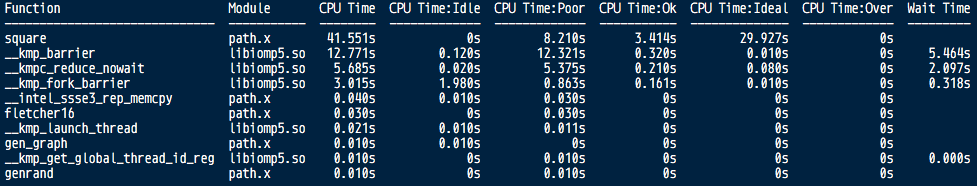
\includegraphics[width=0.7\columnwidth]{amplxe}
			\caption{Most time consuming functions in the base code.}
			\label{amplxe}
		\end{center}
	\end{figure}

\subsection{Scaling}

\section{OpenMPI}

\subsection{Profiling}
\subsection{Scaling}

\section{Processor Offloading}

\section{Additional Changes}
Future, probably also want to test compiler flags, blocking (?)

\section{Overview}

\begin{thebibliography}{1}

\end{thebibliography}

\end{document}